\documentclass[fleqn]{article}
\usepackage[UTF8]{ctex}
\usepackage{listings}
\usepackage{diagbox}
\usepackage[german]{babel}
\usepackage[T1]{fontenc}
\usepackage[latin1]{inputenc}
\usepackage{titlesec}
\usepackage{geometry}
\usepackage{qtree}
\usepackage{tikz}
\usepackage{multirow}
\usepackage{amsmath}
\usepackage{amssymb}
\setcounter{secnumdepth}{0}
\usetikzlibrary{positioning}
\geometry{top=2.5cm, bottom=2.5cm}
\lstset{
 columns=fixed,       
 numbers=left,                                        % 在左侧显示行号
 numberstyle=\tiny\color{gray},                       % 设定行号格式
 frame=none,                                          % 不显示背景边框
 backgroundcolor=\color[RGB]{245,245,244},            % 设定背景颜色
 keywordstyle=\color[RGB]{40,40,255},                 % 设定关键字颜色
 numberstyle=\footnotesize\color{darkgray},           
 commentstyle=\it\color[RGB]{0,96,96},                % 设置代码注释的格式
 stringstyle=\rmfamily\slshape\color[RGB]{128,0,0},   % 设置字符串格式
 showstringspaces=false,                              % 不显示字符串中的空格
 language=c++,                                        % 设置语言
 breaklines,                                          % 自动换行
}

%\title{TU Chemnitz \\ Praktikum Grundlagen Technische Informatik \\ Versuch Sequ1}

%\author{Gruppe 5 - Team 5: \\ Dongze Yang \\Xiangyu Tong \\ Treshchun Kateryna}

\begin{document}

%\maketitle



\newpagestyle{main}{
    \sethead{}{}{Betriebssystem}
    \setfoot{}{\thepage}{}
    \headrule
    \footrule
}
\pagestyle{main}

\section{概念题}

\subsection{ss18}

\textbf{1.} Was sind die zwei Sichten auf das Betriebssystem?操作系统的两种观点是什么?

Das Betriebssystem ist eine virtuelle Maschine und Verwalter von Ressourcen.操作系统是虚拟机和资源管理器。

\textbf{2.} Welches ist kein Grundkonzept in Betriebssystemen?操作系统中哪个不是基本概念?

Dynamik – Fähigkeit, neue Funktionen und Software-Updates zur Laufzeit einzubringen.动态-能够在运行时添加新功能和软件更新

\textbf{3.}Was ist das Konzept eines Mikro-Kern (microkernel)?微内核(microkernel)的概念是什么?

Der Kern umfasst meist nur ein Prozesskonzept und deren Interaktion.核心通常只包含一个流程概念及其交互.

\textbf{4.}Welche der folgenden Aussagen ist korrekt?下列哪种说法是正确的?

Beim automatischen Umschalten müssen kritische Abschnitte durch gegenseitigen Aus-schluss geschützt werden.自动切换时,必须通过互斥来保护关键部分

\textbf{5.}Wann findet eine Verdrängungsprüfung statt?何时进行位移测试?

An allen Übergängen in die Bereitmenge.过渡到现成的数量

\textbf{6.}Wie wird die Scheduling-Strategie ausgewählt?如何选择调度策略?

Abhängig von den Zielen für das Rechnersystem, z.B. Antwortzeit, Durchsatz.根据计算机系统的目标,例如 响应时间,吞吐量

\textbf{7.}Welche der Aussagen zu Multilevel Feedback (FB) ist korrekt?关于多级反馈(FB)的哪些陈述是正确的?

FB Ist eine Standardstrategie mit Zeitscheiben und Verdrängung.FB是具有时间片和位移的标准策略。

\textbf{8.}Was ist der Unterschied zwischen logischem und physischem Adressraum?逻辑和物理地址空间有什么区别?

Der logische Adressraum ist die Repräsentation des Speichers für das laufende Programm,während der physische Adressraum durch den Adresssbus definiert ist.逻辑地址空间代表正在运行的程序的内存,而物理地址空间则由地址总线定义。

\textbf{9.}Welche Aussage zu Wiedereingliederungskonzepten bei der Speicherverwaltung ist korrekt?关于内存管理中的重新集成概念,哪种说法是正确的?

Die Wiedereingliederung erfolgt sofort oder verzögert.重新融合是立即的还是延迟的

\textbf{10.}Bei positionsunabhängigem Code wird…使用与位置无关的代码...

ausschließlich relative Adressierung vorgenommen.仅相对寻址

\textbf{11.}Mehrstufige Seitentabellen haben den Vorteil, dass…多级页表的优点是...

der Speicherbedarf pro Pozess geringer wird.每个进程的内存需求将减少。

\textbf{12.}Was ist Thrashing?什么是颠簸

Die Prozessorauslastung ist schlecht, da das Betriebssystem kontinuierlich Seiten tauscht.处理器利用率很差,因为操作系统不断交换页面。

\textbf{13.}Was ist der funktionale Aspekt der Prozesskooperation?流程合作的功能方面是什么?

Der Zugriff auf gemeinsame Daten.访问共享数据

\textbf{14.}Was realisieren Semaphoren?信号量是做什么的?

Zählersperren für eine kapazitive Beschränkung.计数器锁定以限制电容。

\textbf{15.}Was sind die Coffman-Kriterien?考夫曼准则是什么?

Die Kriterien unter denen eine Verklemmung existiert.存在僵局的条件

\subsection{ss17}

\textbf{1.}Was ist die Stundenglas-Architektur?什么是沙漏架构?

Das Betriebssystem bietet standardisierte Schnittstellen.操作系统提供标准化接口

\textbf{2.}Welche Aussage gilt für ein Micro-Kern (microkernel) Betriebssystem?哪种说法适用于微内核(microkernel)操作系统?

Die Architektur bietet bessere Flexibilität und Erweiterbarkeit als andere Ansätze.与其他方法相比,该体系结构提供了更好的灵活性和可扩展性。

\textbf{3.}Was ist bei der Ausführung von Software im Kernmodus (kernel mode) zu berücksichtigen?在内核模式下运行软件时需要考虑什么?

Die Software kann auf alle Ressourcen und Kacheln zugreifen.该软件可以访问所有资源和图块。

\textbf{4.}Welche Aussage ist für logische Betriebsmittel korrekt?哪种说法对逻辑资源正确?

Logische Betriebsmittel sind eine Abstraktion.逻辑资源是一种抽象。

\textbf{5.}Was findet bei jedem Systemruf statt, der zur Ausführung von Kernel-Code führt?导致内核代码执行的每个系统调用会发生什么?

Ein Scheduling-Vorgang.调度过程

\textbf{6.}Was bewirkt das folgende Kommando in einer Shell: ls -l|grep .tex  Shell中的以下命令做什么:ls -l | grep .tex

Eine Liste der Dateien wird ausgegeben, die genau auf ‘.tex’ enden.输出的文件列表恰好在“ .tex”上结束。

\textbf{7.}Was ist ein kritischer Abschnitt?什么是关键部分?

Ein Abschnitt im Programm, der bei verzahnter nebenläufiger Ausführung zu Problemenführen kann.如果执行并行运行,程序中可能导致问题的部分。

\textbf{8.}Eine Kernsperre schützt implizit einen kritischen Abschnitt, wenn … 如果...,核心锁将隐式保护关键部分。

der Abschnitt im Kernmodus ausgeführt wird.该部分在核心模式下运行。

\textbf{9.}In welchem Fall ist Kernausschluss NICHT nötig?在哪种情况下不需要排除核心?

Einprozessorsystem ohne Interrupts.单处理器系统无中断

\textbf{10.}Alle Threads eines Prozesses teilen sich ...  进程的所有线程共享...

einen gemeinsamen logischen Adressraum.通用逻辑地址空间。

\textbf{11.}Welche Aussage ist für Scheduling mit Highest Response Ratio Next korrekt?哪条陈述对接下来的最高响应率计划是正确的?

Beim Antwortverhältnis wird die Wartezeit des Prozesses mit berücksichtigt.响应率考虑了过程的等待时间

\textbf{12.}Bei relativer Adressierung…随着相对地址...

wird die endgültige Adresse beim Kompilieren des Programmes festgelegt.最终地址在编译程序时确定。

\textbf{13.}Ein Seitenfehler…页面错误...

löst einen Interrupt aus und blockiert den auslösenden Prozess.触发中断并阻止触发过程。

\textbf{14.}Wie viele Seiten gibt es in einem 32-Bit System mit 256 Byte großen Seiten?在具有256字节页面的32位系统中,有多少页面?

$2^{24}$ bzw. 16.777.216 Seiten

\textbf{15.}Welchen Vorteil bringt ein TLB (Translation Lookaside Buffer)?TLB(转换后备缓冲区)的优点是什么?

Die Anzahl der Hauptspeicherzugriffe bei Paging und Segmentierung wird reduziert.分页和分段期间的主内存访问次数减少了。

\textbf{16.}Bei der Auswahlstrategie FIFO im Rahmen der Seitenersetzung…使用页面替换上下文中的选择策略FIFO ...

wird die Seite ausgelagert, welche zuerst eingelagert wurde.最初存储的页面被换出。

\textbf{17.}Wann sind Prozesse potentiell verklemmt?何时可能阻塞进程?

Wenn die vier Coffman-Bedingungen erfüllt sind.当满足四个科夫曼条件时。

\subsection{ss16}

\textbf{1.}Was zeichnet eine Mikrokernelarchitektur im Vergleich zu anderen Architekturen aus?微内核架构与其他架构的区别是什么?

Bessere Ausfallsicherheit.更好的可靠性

\textbf{2.}Was ist ein Prozess?什么是进程?

Ein Programm, welches nicht im Systemmodus ausführbar ist.无法在系统模式下执行的程序。

\textbf{3.}Ein Thread ... 一个线程...

teilt sich den Adressraum mit allen anderen Threads im Prozess.与进程中的所有其他线程共享地址空间。

\textbf{4.}Welche Funktionalitäten muss ein Mikrokernel im Systemmodus implementieren?微内核必须在系统模式下实现哪些功能?

Nebenläufige Ausführung und Interprozesskommunikation.并发执行和进程间通信

\textbf{5.}Welche Aussage ist korrekt?哪种说法正确?

Nebenläufigkeit und Parallelität haben nichts miteinander zu tun.并发和并行性彼此无关。

\textbf{6.}Caching ...缓存...

nutzt das Lokalitätsprinzip aus.缓存利用了本地性原则。

\textbf{7.}Was versteht man üblicherweise unter dem Begriff “Terminal”?术语“终端”通常是什么意思?

Einen speziellen Modus des Betriebssystems für administrative Aufgaben.用于管理任务的操作系统的一种特殊模式。

\textbf{8.}Verdrängte Prozesse gelangen in den Zustand ... 被压制的进程进入状态...

"wartend"“等候”

\textbf{9.}Beim Scheduling nach FCFS können Prozesse ... 根据FCFS进行调度时,处理...

nicht in den “wartend” - Zustand wechseln.根据FCFS进行调度时,进程无法切换到“等待”状态。

\textbf{10.}Welche Aussage trifft für das preemptive Round-Robin Scheduling zu?哪条语句适用于抢占式循环调度?

Ein Quantum, welches größer ist als die kleinste Job-Ausführungszeit, macht den Ansatzäquivalent zu FCFS.大于最小作业执行时间的量会使该方法等效于FCFS。

\textbf{11.}In welchem Fall ist Kernausschluss NICHT nötig?在哪种情况下不需要排除核心?

Einprozessorsystem ohne Interrupt.单处理器系统无中断

\textbf{12.}Wenn es im bisherigen Verlauf der Ausführung für eine Prozessmenge eine sichere Betriebsmittelsituation gab, dann ... 如果到目前为止,在执行过程中存在安全的设备数量,那么...

kann es in der weiteren Ausführung zu einer Verklemmung kommen.在进一步执行中可能会发生卡纸。

\textbf{13.}Welche Zustandsformen von Betriebsmitteln gibt es?有哪些类型的设备状况?

real, virtuell, partiell.真实,虚拟,局部

\textbf{14.}Interner Verschnitt ...  内部垃圾...

minimiert den Speicherbedarf des Kerns. 内部浪费最大程度地减少了内核的内存需求。

\textbf{15.}Wenn in der Speicherverwaltung Reststücke der Anforderung zugeschlagen werden, dann \dots 如果将需求的剩余部分添加到存储管理中,则

tritt nur noch externer Verschnitt auf. 则只会发生外部浪费。

\textbf{16.}Welche Aussage ist richtig?哪个说法正确?

Eine MMU übersetzt logische Adressen in physische Adressen.MMU将逻辑地址转换为物理地址。

\textbf{17.}Wieviel Speicher ist für die einstufige Seitentabelle eines 32-Bit-Prozess mit 4 kiByte Seitengröße mindestens erforderlich?页大小为4 kiByte的32位进程的单级页表所需的最小内存是多少?

4 kiByte 千字节

\section{简答题}

\noindent\textbf{Aufgabe ss18-A2:}
Gegeben sei folgendes Prozessszenario:给出以下处理方案:

\begin{center}
    \begin{tabular}{|c|c|c|c|}
        \hline
        Prozess&Bedinzeit $t_s$&Ankunftzeit $t_a$&Priorität $p$\\
        \hline
        A&6&0&1(niedrigste)\\
        B&4&3&2\\
        C&5&2&3\\
        D&2&7&4(höchste)\\
        \hline
    \end{tabular}
\end{center}

\indent Erstellen Sie Ausführungspläne für die folgenden Scheduling-Strategien.为以下调度策略创建执行计划。

\indent (a)RR(2) - Round-Robin mit Zeitscheibe in der Größe 2.时间片大小为2的轮循

\indent Hinweis: Neu ankommende Prozesse werden \textbf{am Ende} der Warteschlange, 
allerdings \textbf{vor} gerade verdrängten Prozessen eingereiht.注意:新到达的进程位于队列的末尾,但在刚被替换的进程之前。

\begin{center}
    \begin{tabular}{|c||c|c|c|c|c|c|c|c|c|c|c|c|c|c|c|c|c|c|c|}
        \hline
        t&0&1&2&3&4&5&6&7&8&9&10&11&12&13&14&15&16&17&18\\
        \hline
        A&+&+&&&+&+&&&&&+&+&&&&&&&\\
        \hline
        B&&&&&&&+&+&&&&&&&&&&&\\
        \hline
        C&&&+&+&&&&&+&+&&&&&+&+&+&&\\
        \hline
        D&&&&&&&&&&&&&+&+&&&&&\\
        \hline
    \end{tabular}
\end{center}

\indent (b)PRIO-P - Priorities Preemptive优先抢先

\begin{center}
    \begin{tabular}{|c||c|c|c|c|c|c|c|c|c|c|c|c|c|c|c|c|c|c|c|}
        \hline
        t&0&1&2&3&4&5&6&7&8&9&10&11&12&13&14&15&16&17&18\\
        \hline
        A&+&+&&&&&&&&&&&&+&+&+&+&&\\
        \hline
        B&&&&&&&&&&+&+&+&+&&&&&&\\
        \hline
        C&&&+&+&+&+&+&&&&&&&&&&&&\\
        \hline
        D&&&&&&&&+&+&&&&&&&&&&\\
        \hline
    \end{tabular}
\end{center}

\noindent\textbf{Aufgabe ss17-A2:}
Gegeben sei folgendes Prozessszenario:

\begin{center}
    \begin{tabular}{|c|c|c|c|}
        \hline
        Prozess&Bedinzeit $t_s$&Ankunftzeit $t_a$&Priorität $p$\\
        \hline
        A&5&3&1(niedrigste)\\
        B&3&6&2\\
        C&7&0&3\\
        D&4&4&4(höchste)\\
        \hline
    \end{tabular}
\end{center}

\indent Erstellen Sie Ausführungspläne für die folgenden Scheduling-Strategien.

\indent (a)RR(3) - Round-Robin mit Zeitscheibe in der Größe 3.时间片大小为3的轮循

\indent Hinweis: Neu ankommende Prozesse werden \textbf{am Ende}
 der Warteschlange, allerdings \textbf{vor} gerade verdrängten Prozessen eingereiht.

\begin{center}
    \begin{tabular}{|c||c|c|c|c|c|c|c|c|c|c|c|c|c|c|c|c|c|c|c|}
        \hline
        t&0&1&2&3&4&5&6&7&8&9&10&11&12&13&14&15&16&17&18\\
        \hline
        A&&&&+&+&+&&&&&&&&&&+&+&&\\
        \hline
        B&&&&&&&&&&&&&+&+&+&&&&\\
        \hline
        C&+&+&+&&&&+&+&+&&&&&&&&&+&\\
        \hline
        D&&&&&&&&&&+&+&+&&&&&&&+\\
        \hline
    \end{tabular}
\end{center}

(b) SRTN - Shortest Remaining Time Next.剩余时间最短

\begin{center}
    \begin{tabular}{|c||c|c|c|c|c|c|c|c|c|c|c|c|c|c|c|c|c|c|c|}
        \hline
        t&0&1&2&3&4&5&6&7&8&9&10&11&12&13&14&15&16&17&18\\
        \hline
        A&&&&&&&&&&&&&&&+&+&+&+&+\\
        \hline
        B&&&&&&&&+&+&+&&&&&&&&&\\
        \hline
        C&+&+&+&+&+&+&+&&&&&&&&&&&&\\
        \hline
        D&&&&&&&&&&&+&+&+&+&&&&&\\
        \hline
    \end{tabular}
\end{center}

(c) PRIO-NP - Priorities Nonpreemptive.优先级非抢占

\begin{center}
    \begin{tabular}{|c||c|c|c|c|c|c|c|c|c|c|c|c|c|c|c|c|c|c|c|}
        \hline
        t&0&1&2&3&4&5&6&7&8&9&10&11&12&13&14&15&16&17&18\\
        \hline
        A&&&&&&&&&&&&&&&&&&&\\
        \hline
        B&&&&&&&&&&&&&&&&&&&\\
        \hline
        C&&&&&&&&&&&&&&&&&&&\\
        \hline
        D&&&&&&&&&&&&&&&&&&&\\
        \hline
    \end{tabular}
\end{center}

\noindent\textbf{Aufgabe ss16-A3:}
题干同上。

\begin{center}
    \begin{tabular}{|c|c|c|c|}
        \hline
        Prozess&Bedinzeit $t_s$&Ankunftzeit $t_a$&Priorität $p$\\
        \hline
        A&7&6&1(niedrigste)\\
        B&4&0&2\\
        C&3&4&3\\
        D&5&3&4(höchste)\\
        \hline
    \end{tabular}
\end{center}

(a) RR(2)

\begin{center}
    \begin{tabular}{|c||c|c|c|c|c|c|c|c|c|c|c|c|c|c|c|c|c|c|c|}
        \hline
        t&0&1&2&3&4&5&6&7&8&9&10&11&12&13&14&15&16&17&18\\
        \hline
        A&&&&&&&&&+&+&&&&+&+&&+&+&+\\
        \hline
        B&+&+&+&+&&&&&&&&&&&&&&&\\
        \hline
        C&&&&&&&+&+&&&&&+&&&&&&\\
        \hline
        D&&&&&+&+&&&&&+&+&&&&+&&&\\
        \hline
    \end{tabular}
\end{center}

(b) LCFS-PR

\begin{center}
    \begin{tabular}{|c||c|c|c|c|c|c|c|c|c|c|c|c|c|c|c|c|c|c|c|}
        \hline
        t&0&1&2&3&4&5&6&7&8&9&10&11&12&13&14&15&16&17&18\\
        \hline
        A&&&&&&&+&+&+&+&+&+&+&&&&&&\\
        \hline
        B&+&+&+&&&&&&&&&&&&&&&&+\\
        \hline
        C&&&&&+&+&&&&&&&&+&&&&&\\
        \hline
        D&&&&+&&&&&&&&&&&+&+&+&+&\\
        \hline
    \end{tabular}
\end{center}

(c) PRIO-P

\begin{center}
    \begin{tabular}{|c||c|c|c|c|c|c|c|c|c|c|c|c|c|c|c|c|c|c|c|}
        \hline
        t&0&1&2&3&4&5&6&7&8&9&10&11&12&13&14&15&16&17&18\\
        \hline
        A&&&&&&&&&&&&&+&+&+&+&+&+&+\\
        \hline
        B&+&+&+&&&&&&&&&+&&&&&&&\\
        \hline
        C&&&&&&&&&+&+&+&&&&&&&&\\
        \hline
        D&&&&+&+&+&+&+&&&&&&&&&&&\\
        \hline
    \end{tabular}
\end{center}


\noindent\textbf{Aufgabe ss18-A3:} Ein Speicher von 16 MiByte1 werde nach dem Buddy-Verfahren verwaltet. Die kleinste Blockgröße betrage 512 kiByte. Folgende Speicheranforderungen bzw. -freigaben treffen der Reihe nach ein.
使用伙伴方法管理16 MiByte1的内存。 最小块大小为512 KB。 以下存储请求和发布是按顺序进行的。

(i) Anforderung von 2 MiByte 需求

(ii) Anforderung von 20 kiByte 

(iii) Anforderung von 5 MiByte 

(iv) Anforderung von 1,5 MiByte 

(v) Anforderung von 1,9 MiByte 

(vi) Freigabe der Anforderung (ii)  释放请求

(vii) Freigabe der Anforderung (iv)
\\
\\
\indent (a)Stellen Sie die Speicherbelegung nach jedem Anforderungs- bzw. Freigabeschritt dar, so wie sie sich aus der Anwendung des Buddy-Verfahrens ergibt.
在每个请求或释放步骤之后显示内存分配,这是由于应用了伙伴程序导致的。

(b)Was würde passieren, wenn im Anschluss an (vii) eine Speicheranforderung von 3 MiByte gestellt wird? Begründen Sie.
在(vii)之后发出3 MiByte的存储请求会怎样? 说明。

\begin{center}
    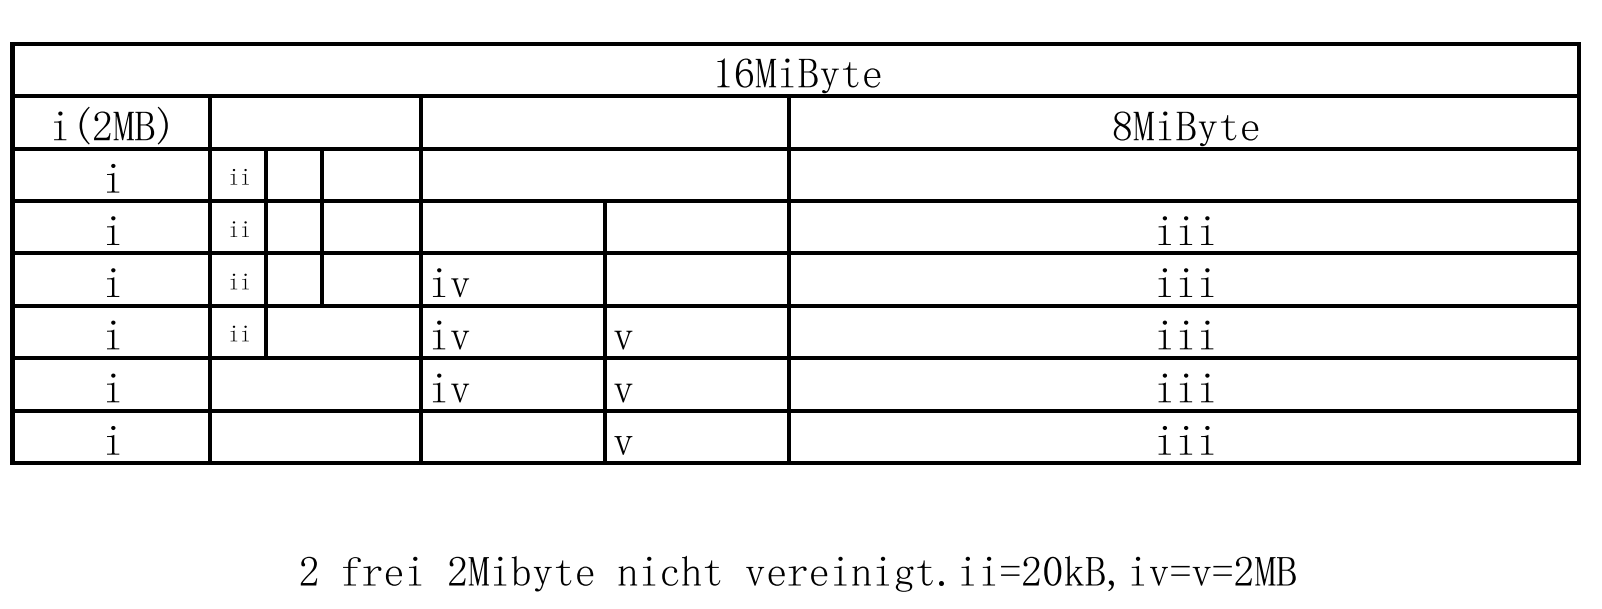
\includegraphics[scale=0.2]{bild2.png}
\end{center}

\noindent\textbf{Aufgabe ss17-A3:}

(a) Ergänzen Sie in den Kreisen die möglichen Zustände eines Prozesses.在圈子中完成过程的可能状态。

(b) Ergänzen Sie die Bezeichnungen der Zustandsübergänge.完成状态转换的名称。

\begin{center}
    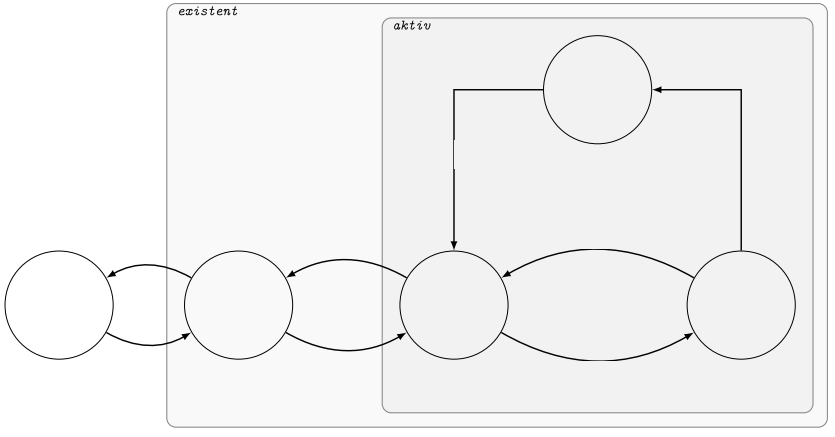
\includegraphics[scale=0.5]{bild1.png}
\end{center}

(c) Bei welchen Zustandsübergängen findet möglicherweise eine Verdrängungsprüfung (\textit{check for preemption}) statt? Begründen Sie!
可以在哪个状态转换中进行抢占检查? 说明!

\textbf{Ans:}

(a)(b): \begin{center}
    
\includegraphics[scale=0.6]{bild4.png}
\end{center}

(c) ready $\rightarrow$ running: Verdrängungsprüfung 位移测试

\noindent\textbf{Aufgabe ss18-A4:}

In einem System wird zur effektiven Speicherverwaltung und zum Speicherschutz eine einstufige Segmentierung verwendet.
在系统中,单步分段用于有效的内存管理和内存保护。

Der Addressraum$^2$ des Systems ist 2 MiByte (1MiByte = $2^{20}$ Byte) groß, die Segmenttabelle 4 KiByte (1 KiByte = $2^{10}$ Byte), die Adressierung erfolgt byteweise.
系统的地址空间$ ^2 $为2 MiByte(1MiByte = $ 2^{20} $ Byte),段表为4 KiByte(1 KiByte = $ 2^{10} $ Byte),寻址是逐字节进行的。

Wie groß ist maximal ein Segment?段的最大大小是多少?

\textbf{Ans:}

System: 2 MiByte = $2^{21}$ Byte $\Rightarrow$ 21 Bit notwendig für eine Adresse.
系统:2 MiByte = $ 2^{21} $ Byte $ \Rightarrow $ 21位是地址所必需的

Segmenttabelle: 4 KiByte = $2^{10}$ Byte $\Rightarrow$ 10 Bit.
段表:4 KiByte = $ 2^{10} $ Byte $ \Rightarrow $ 10 bit

\begin{center}
    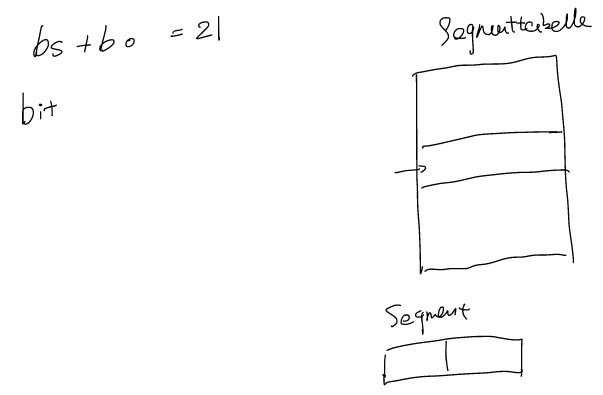
\includegraphics[scale = 0.4]{bild3.png}
\end{center}
\noindent\textbf{Aufgabe ss18-A5:}

Ein Algorithmus ermögliche den gegenseitigen Ausschluss zwischen \textbf{genau zwei} Prozessen 
(z.B. der Peterson-Algorithmus). Die kritischen Abschnitte werden dabei durch die 
Funktionspaare enter\_A($L$) / leave\_A($L$) und enter\_B($L$) / leave\_B($L$) geklammert, 
wobei $L$ die Datenstruktur der Sperre darstellt.

一种算法可实现\textbf {恰好两个}进程之间的互斥
(例如Peterson算法)。 关键部分由
函数对在括号内 输入\_A($ L $)/ 离开\_A($ L $),然后在括号中 输入\_B($ L $)/ 离开\_B($ L $),
其中$ L $表示锁的数据结构。


\begin{center}
    \begin{tabular}{l|l}
        $P_1$&$P_2$\\
        \textbf{enter\_A($L$)}&\textbf{enter\_B($L$)}\\
        $\vdots$&$\vdots$\\
        \textit{kritischer Abschnitt von Prozess 1}&\textit{kritischer Abschnitt von Prozess 2}\\
        $\vdots$&$\vdots$\\
        \textbf{leave\_A($L$)}&\textbf{leave\_B($L$)}
    \end{tabular}
\end{center}

Eine Erweiterung des Algorithmus auf mehr als zwei Prozesse ist jedoch nicht auf einfache Weise möglich. Für eine Lösung mit drei Prozessen, wurde daher auf zwei Sperrobjekte zurückgegriffen, die wie folgt benutzt werden.
但是,很难将算法扩展到两个以上的过程。 对于具有三个进程的解决方案,使用了两个锁定对象,其使用情况如下。

\begin{center}
    \begin{tabular}{l|l|l}
        $P_1$&$P_2$&$P_3$\\
        \textbf{enter\_A($L_1$)}&\textbf{enter\_B($L_1$)}\\
        &\textbf{enter\_A($L_2$)}&\textbf{enter\_B($L_2$)}\\
        $\vdots$&$\vdots$&$\vdots$\\
        \textit{kritischer Abschnitt von Prozess 1}&\textit{kritischer Abschnitt von Prozess 2}&\textit{kritischer Abschnitt von Prozess 2}\\
        $\vdots$&$\vdots$&$\vdots$\\
        &\textbf{leave\_A($L_2$)}&\textbf{leave\_B($L_2$)}\\
        \textbf{leave\_A($L_1$)}&\textbf{leave\_B($L_1$)}
    \end{tabular}
\end{center}

(a)Die obige Konstruktion ist fehlerhaft. Zeigen Sie, unter welchen Bedingungen es zu einem fehlerhaften Verhalten kommen kann und begründen Sie kurz.
上述构造有缺陷。 显示发生错误行为的条件并给出简要说明。

(b)Was bedeuten die Begriffe "Sicherheit" und "Lebendigkeit" in Bezug auf den gegenseitigen Ausschluss?
关于相互排斥,“安全”和“活力”是什么意思?

(c)Wie müsste die obige Lösung ergänzt werden, damit eine sichere und lebendige Lösung für den gegenseitigen Ausschluss entsteht?
如何对上述解决方案进行补充,以创建安全生动的互斥解决方案?

\textbf{Ans:} 

(a)Wenn $P_1$ und $P_3$ gleichzeitig in kritische Abschnitte eintreten wollen, wird der gegenseitigen Ausschluss zwischen Ihnen nicht realisiert, den sowohl die Sperre $L_1$ so wie $L_2$ frei sind.
如果$ P_1 $和$ P_3 $要同时进入关键部分,则不会实现您之间的互斥,因为锁$ L_1 $和$ L_2 $都是免费的。

(b)

Sicherheit: Zu einer Zeit darf sich höchstens ein einziger Prozess in einem kritischen Abschnitt desselben Betriebsmittels befinden.
同一设备的关键部分最多只能进行一个进程。

Lebendigkeit: Jedem Prozess, der einen kritischen Abschnitt betreten will, muss dies irgendwann gelingen.
每个想要进入关键部分的进程都必须在某个时候成功。

(c)
\\
\\
\\
\\
\\
\\
\noindent\textbf{Aufgabe ss17-A5:}

Die folgende Softwarelösung soll den gegenseitigen Ausschluss zweier Threads $T1$ und $T2$
 in einem kritischen Abschnitt realisieren. Jede Ausführung einer Zeile ist atomar, dazwischen kann jederzeit eine Umschaltung stattfinden.

以下软件解决方案旨在在关键部分中实现两个线程$ T1 $和$ T2 $的互斥。 每条线的执行都是原子性的,在两者之间可以随时进行切换。

\begin{center}
    \begin{tabular}{l|l}
        $T_1$&$T_2$\\
        \multicolumn{2}{c}{int var1 = 0; int var2 = 0;}\\
        var1 = 1; & var2 = 1;\\
        do \{\} while(var2 == 1);& do \{\} while (var1 == 1);\\
        /*\textit{Beginn kritischer Abschnitt}*/&/*\textit{Beginn kritischer Abschnitt}*/\\
        /*\dots*/&/*\dots*/\\
        /*\textit{Ende kritischer Abschnitt}*/&/*\textit{Ende kritischer Abschnitt}*/\\
        var1 = 0; & var2 = 0;
    \end{tabular}
\end{center}

(a) Stellt die Lösung den gegenseitigen Ausschluss in jedem Fall sicher? Wenn ja, wieso? Wenn nein, beschreiben Sie ein Gegenbeispiel.
该解决方案在任何情况下是否确保相互排斥? 如果是这样,为什么? 如果否,请描述一个反例。

(b) Stellt die Lösung die Lebendigkeit (\textit{liveliness}) der Threads sicher? Wenn ja, wieso? Wenn nein, beschreiben Sie ein Gegenbeispiel.
解决方案是否确保线程的生动性(\textit {liveliness})? 如果是这样,为什么? 如果否,请描述一个反例。

\textbf{Ans:}

(a) 可以,但有可能饿死。

(b) Nein $\Rightarrow T_1: var1 = 1\rightarrow T_2: var2 = 1\rightarrow T_2: do \{\}while$ is true $\rightarrow T_1: do\{\}while$ is true. 陷入无限循环。饿死。

\noindent\textbf{Aufgabe ss16-A2:}

Folgende Ansätze sollen theoretisch den gegenseitigen Ausschluss zweier Prozesse $P_1$ und $P_2$ realisieren. Jede Zeile wird als atomarer Schritt ausgeführt, der Scheduler kann jederzeit nach solch einem Schritt eine Prozessumschaltung veranlassen. Erläutern Sie jeweils für jeden Ansatz:
以下方法在理论上应实现两个进程$ P_1 $和$ P_2 $的互斥。 每行都是一个原子步骤,调度程序可以在该步骤之后的任何时间启动进程切换。 对于每种方法,请说明:

1. Ist der gegenseitige Ausschluss garantiert? 是否保证互斥?

2. Ist Verklemmungsfreiheit garantiert? 是否可以保证无死锁?

3. Welche Coffmann-Bedingungen werden ggf. NICHT erfüllt? 哪些科夫曼条件可能无法满足?

4. Ist Verhungern unmöglich?饥饿是不可能的吗?

\begin{center}
    \begin{tabular}{l|l}
        $P_1$&$P_2$\\
        \multicolumn{2}{c}{int var = 0;}\\
        while(1)\{&while(1)\{\\
        \qquad while(var == 1)\{\};&\qquad while (var == 1)\{\};\\
        \qquad var = 1&\qquad var = 1\\
        \qquad /*\dots*/&\qquad /*\dots*/\\
        \qquad /*\textit{Kritischer Abschnitt}*/&\qquad /*\textit{Kritischer Abschnitt}*/\\
        \qquad /*\dots*/&\qquad /*\dots*/\\
        \qquad var = 0;&\qquad var = 0;\\
        \}&\}
    \end{tabular}
\end{center}

(b)

\begin{center}
    \begin{tabular}{l|l}
        $P_1$&$P_2$\\
        \multicolumn{2}{c}{int var1 = 0; int var2 = 0;}\\
        while(1)\{&while(1)\{\\
        \qquad m1: var1 = 1;&\qquad m2: var2 = 1;\\
        \qquad if(var2 == 1)&\qquad if(var1 == 1)\\
        \qquad \{&\qquad \{\\
        \qquad\qquad var1 = 0;&\qquad\qquad var2 = 0;\\
        \qquad\qquad goto m1;&\qquad\qquad goto m2;\\
        \qquad \}&\qquad \}\\
        \qquad /*\dots*/&\qquad /*\dots*/\\
        \qquad /*\textit{Kritischer Abschnitt}*/&\qquad /*\textit{Kritischer Abschnitt}*/\\
        \qquad /*\dots*/&\qquad /*\dots*/\\
        \qquad var1 = 0;&\qquad var2 = 0;\\
        \}&\}
    \end{tabular}
\end{center}

(c)

\begin{center}
    \begin{tabular}{l|l}
        $P_1$&$P_2$\\
        \multicolumn{2}{c}{int var1 = 0; int var2 = 0;}\\
        while(1)\{&while(1)\{\\
        \qquad var1 = 1;&\qquad var2 = 1;\\
        \qquad while(var2 == 1)\{\};&\qquad while (var1 == 1)\{\};\\
        \qquad /*\dots*/&\qquad /*\dots*/\\
        \qquad /*\textit{Kritischer Abschnitt}*/&\qquad /*\textit{Kritischer Abschnitt}*/\\
        \qquad /*\dots*/&\qquad /*\dots*/\\
        \qquad var1 = 0;&\qquad var2 = 0;\\
        \}&\}
    \end{tabular}
\end{center}







\noindent\textbf{Aufgabe ss18-A6:}

Folgendes Stück C-Code benutzt die UNIX-Systemrufe fork() und waitpid(). 
Weiterhin sind sem\_init(), sem\_up() und sem\_down() die klassischen Semaphor-Operationen. 
Die Funktion sem\_open() erzeuge eine “named Semaphor”. 
Der zweite Parameter gibt den Ausgangswert der Semaphor an.

以下C代码使用UNIX系统调用fork()和waitpid()。
此外,sem\_init(),sem\_up()和sem\_down()是经典的信号量操作。
函数sem\_open()创建一个“命名信号量”。
第二个参数指定信号量的初始值。

\begin{lstlisting}
int main()
{
    pid_t p1, p2; 
    sem_t *s;

    s = sem_open("NAMED_SEMAPHOR", 0);

    p1 = fork(); 
    wait(NULL);
    if(p1 == 0) 
    {
        p2 = fork(); 
        wait(NULL);
        if(p2 > 0) 
        {
            printf("S\n"); 
            sem_up(s);
        }
        else 
        {
            sem_down(s); 
            printf("R\n"); 
            sem_up(s);
        } 
    }
    else 
    {
        sem_down(s); 
        printf("A\n"); 
        sem_up(s);
    } 

    return 0;
}
\end{lstlisting}

(a) Zeichnen Sie ein Ablaufdiagramm für dieses Programm, in das alle Systemrufe, Ausgaben und Semaphor-Operationen inkl. Quellcodezeilennummer eingetragen sind (die Namen reichen aus, Parameter müssen nicht angegeben werden).
绘制该程序的流程图,在其中输入所有系统调用,输出和信号灯操作,包括源代码行号(名称足够,不必指定参数)。

(b)Welche Ausgabe erzeugt das Programm? Begründen Sie!程序生成什么输出? 说明!

\noindent\textbf{Aufgabe ss17-A6:}

Jede der unten dargestellten Funktionen wird durch einen Thread abgearbeitet. 
Die Signale $s1$ bis $s4$ seien global vereinbart.

下面显示的每个功能都由一个线程处理。
信号$ s1 $到$ s4 $在全球范围内已达成共识。

\begin{center}
    \begin{tabular}{l|l}
        void thread\_a()&void thread\_b()\\
        \{&\{\\
        \qquad unsigned int i;&\qquad unsigned int i;\\
        \\
        \qquad for(i = 1; i <= 8; i = i + 4) &\qquad for(i = 2; i <= 8; i = i + 4)\\
        \qquad \{&\qquad \{\\
        \qquad\qquad signal(s2);&\qquad\qquad signal(s1);\\
        \qquad\qquad wait(s1);&\qquad\qquad wait(s2);\\
        \\
        \qquad\qquad /*\textit{Ausgabe von i}*/&\qquad\qquad /*\textit{Ausgabe von i}*/\\
        \qquad\qquad printf("\%d ",i);&\qquad\qquad printf("\%d ",i);\\
        \\
        \qquad\qquad signal(s4);&\qquad\qquad signal(s3);\\
        \qquad\qquad wait(s3);&\qquad\qquad wait(s4);\\
        \\
        \qquad\qquad /*\textit{Ausgabe von i+2}*/&\qquad\qquad /*\textit{Ausgabe von i+2}*/\\
        \qquad\qquad printf("\%d ",i+2);&\qquad\qquad printf("\%d ",i+2);\\
        \qquad\}&\qquad\}\\
        \}&\}
    \end{tabular}
\end{center}

Welche der folgenden Ausgaben können bei Abarbeitung des Programms entstehen und welche nicht?在处理程序时,以下哪些费用可能会产生或可能不会产生?

(i) 1 2 3 4 5 6 7 8

(ii) 2 1 4 3 5 7 6 8

(iii) 1 3 5 7 2 4 6 8

\textbf{Ans:}(i) (ii) ja, (iii) nein.

\noindent\textbf{Aufgabe ss18-A7:}

Ein System unterteilt den physischen Hauptspeicher in vier Kacheln, welche zu Beginn leer sind. Es finden Zugriffe auf Seiten in der folgenden Reihenfolge statt:
系统将物理主内存划分为四个块,这些块最初是空的。 页面按以下顺序访问:
$$1\quad2\quad3\quad4\quad5\quad1\quad2\quad5\quad3\quad4\quad2\quad1\quad3$$

Ergänzen Sie für das Ersetzungverfahren LRU (Least Recently Used) die Belegung 
der Kacheln nach jedem Seitenzugriff. 
Tragen sie dafür die Seitennummern in die jeweiligen Kästchen ein. 
Markieren sie zusätzlich die Zeitpunkte, bei denen ein Seitenzugriffsfehler (\textit{page fault}) auftritt.

对于替换过程LRU(最近最少使用),请在每次访问页面后添加磁贴的分配。 
为此,请在相应的框中输入页码。 同时标记发生页面访问错误(\textit {page fault})的时间。

Hinweis: Das Einlagern in eine leere Kachel wird \textbf{nicht} als Seitenzugriffsfehler gewertet.
注意:\textbf{nicht}放置在一个空白的图块中被认为是页面访问错误。

\begin{center}
    \begin{tabular}{|l|l|l|l|l|l|l|l|l|l|l|l|l|l|l|}
        \hline
        \diagbox{Kachel}{Seite}&1&2&3&4&5&1&2&5&3&4&2&1&3\\        
        \hline
        3&&&&4&4&4&4&4&3&3&3&3&3\\
        \hline
        2&&&3&3&3&3&2&2&2&2&2&2&2\\
        \hline
        1&&2&2&2&2&1&1&1&1&4&4&4&4\\
        \hline
        0&1&1&1&1&5&5&5&5&5&5&5&1&1\\
        \hline
        Seitenzugriffsfehler?&&&&&*&*&*&&*&*&&*&\\
        \hline
    \end{tabular}
\end{center}

\noindent\textbf{Aufgabe ss17-A4:}

题干同上。

(a) FIFO - First In First Out:

\begin{center}
    \begin{tabular}{|l|l|l|l|l|l|l|l|l|l|l|l|l|l|l|}
        \hline
        \diagbox{Kachel}{Seite}&1&2&3&4&5&1&2&5&3&4&2&1&3\\        
        \hline
        3&-&-&-&4&4&4&4&4&3&3&3&3&3\\
        \hline
        2&-&-&3&3&3&3&2&2&2&2&2&2&2\\
        \hline
        1&-&2&2&2&2&1&1&1&1&1&1&1&1\\
        \hline
        0&1&1&1&1&5&5&5&5&5&4&4&4&4\\
        \hline
        Seitenzugriffsfehler?&&&&&*&*&*&&*&*&&&\\
        \hline
    \end{tabular}
\end{center}

(b) LFU - Least Frequently Used:最少使用:

\begin{center}
    \begin{tabular}{|l|l|l|l|l|l|l|l|l|l|l|l|l|l|l|}
        \hline
        \diagbox{Kachel}{Seite}&1&2&3&4&5&1&2&5&3&4&2&1&3\\        
        \hline
        3&-&-&-&4&4&$4^1$&$4^1$&$4^1$&$3^2$&$3^2$&$3^2$&$3^2$&$3^3$\\
        \hline
        2&-&-&3&3&3&$3^1$&$2^2$&$2^2$&$2^2$&$2^2$&$2^3$&$2^3$&$2^3$\\
        \hline
        1&-&2&2&2&2&$1^2$&$1^2$&$1^2$&$1^2$&$4^2$&$4^2$&$4^2$&$4^2$\\
        \hline
        0&1&1&1&1&5&$5^1$&$5^1$&$5^2$&$5^2$&$5^2$&$5^2$&$1^3$&$1^3$\\
        \hline
        S.zug.f?&&&&&*&*&*&&*&*&&*&\\
        \hline
    \end{tabular}
\end{center}

\noindent\textbf{Aufgabe ss16-A5:}
题干同上。

$$1\qquad2\qquad3\qquad4\qquad5\qquad1\qquad3\qquad5\qquad2\qquad3\qquad5\qquad4\qquad5$$

(a) FIFO:

\begin{center}
    \begin{tabular}{|l|l|l|l|l|l|l|l|l|l|l|l|l|l|l|}
        \hline
        \diagbox{Kachel}{Seite}&1&2&3&4&5&1&3&5&2&3&5&4&5\\        
        \hline
        3&&&&4&4&4&4&4&4&3&3&3&3\\
        \hline
        2&&&3&3&3&3&3&3&2&2&2&2&2\\
        \hline
        1&&2&2&2&2&1&1&1&1&1&1&1&5\\
        \hline
        0&1&1&1&1&5&5&5&5&5&5&5&4&4\\
        \hline
        Seitenzugriffsfehler?&&&&&*&*&&&*&*&&*&\\
        \hline
    \end{tabular}
\end{center}

(b) LRU:

\begin{center}
    \begin{tabular}{|l|l|l|l|l|l|l|l|l|l|l|l|l|l|l|}
        \hline
        \diagbox{Kachel}{Seite}&1&2&3&4&5&1&3&5&2&3&5&4&5\\        
        \hline
        3&&&&4&4&4&4&4&2&2&2&2&2\\
        \hline
        2&&&3&3&3&3&3&3&3&3&3&3&3\\
        \hline
        1&&2&2&2&2&1&1&1&1&1&1&4&4\\
        \hline
        0&1&1&1&1&5&5&5&5&5&5&5&5&5\\
        \hline
        Seitenzugriffsfehler?&&&&&*&*&&&*&&&*&\\
        \hline
    \end{tabular}
\end{center}

\noindent\textbf{Aufgabe ss18-A8:} Ein System besteht aus 4 Betriebsmittelklassen und 5 Prozessen.一个系统包含4个资源类和5个过程。

(a)Befindet sich das System mit folgender Betriebsmittelsituation in einem sicheren Zustand?:系统处于以下设备状况下是否处于安全状态?:
$$\vec{v}=(6,7,12,12)\qquad \vec{f}=(2,1,0,0)$$
$$A=\begin{pmatrix}
    0&0&1&2\\
    2&7&5&0\\
    6&6&5&6\\
    4&3&5&6\\
    0&6&5&2
\end{pmatrix}\qquad
B=\begin{pmatrix}
    0&0&1&2\\
    2&0&0&0\\
    0&0&3&4\\
    2&3&5&4\\
    0&3&3&2
\end{pmatrix}$$

(b) Prozess drei fordert, ausgehend vom Initialszustand, eine Instanz des BM Nr. 2. 进程3根据初始状态,请求实例2号BM。

\indent Bestimmen Sie die Art des Zustandes (unsicher, sicher, verklemmt), wenn das System diese Anforderung zulässt.如果系统允许此条件,请确定条件的类型(不安全,安全,卡住)。

\noindent\textbf{Aufgabe ss17-A7:}

Gegeben seien vier Prozesse ($P_1, P_2, P_3, P_4$) und drei Sorten von Ressourcen ($R_1, R_2, R_3$), 
wobei es von $R_1$ insgesamt 9 Exemplare gibt, von $R_2$ gibt es 3 Exemplare und von $R_3$ 6 Exemplare.
给定四个进程($ P_1,P_2,P_3,P_4 $)和三种资源($ R_1,R_2,R_3 $),$ R_1 $有9个副本,$ R_2 $有3个副本,$ R_3 $有6个副本。

Tabelle 1 gibt an, wieviel Exemplare jeder Ressource ein Prozess im Laufe seiner gesamten Lebenszeit anfordert.
表1显示了一个进程在其整个生命周期中请求每个资源的副本数。

\begin{center}
    \begin{tabular}{c|cccc}
        &$R_1$&$R_2$&$R_3$&\\
        \hline
        $P_1$&3&2&2\\
        $P_2$&6&1&3\\
        $P_3$&3&1&4\\
        $P_4$&4&2&2\\
    \end{tabular}\qquad (\textbf{Tabelle 1})
\end{center}

Zu einem gegebenen Zeitpunkt $t$ belegen die Prozesse jeweils die in Tabelle 2 angegebenen Anzahl von Ressourcen.
在给定的时间$ t $,每个进程占用表2中指定的资源数量。

\begin{center}
    \begin{tabular}{c|cccc}
        &$R_1$&$R_2$&$R_3$&\\
        \hline
        $P_1$&1&0&0\\
        $P_2$&5&1&1\\
        $P_3$&2&1&1\\
        $P_4$&0&0&2\\
    \end{tabular}\qquad (\textbf{Tabelle 2})
\end{center}

(a) Führen sie den Matrixalgorithmus für den Zeitpunkt $t$ durch und erläutern Sie Ihre Schritte.
对时间$ t $执行矩阵算法,并解释您的步骤。

(b) Was sagt das Ergebnis aus?结果说明什么?

\textbf{Ans:}

$$\vec{v} = (R_1,R_2,R_3) = (9,3,6)$$

$$B=\begin{pmatrix}
   1&0&0\\
   5&1&1\\
   2&1&1\\
   0&0&2 
\end{pmatrix}\qquad A=\begin{pmatrix}
    3&2&2\\
    6&1&3\\
    3&1&4\\
    4&2&2
\end{pmatrix}\qquad R=A-B = \begin{pmatrix}
    2&2&2\\
    1&0&2\\
    1&0&3\\
    4&2&0
\end{pmatrix}$$

$$\vec{r_2}=R_2=(1,0,2)<\vec{f}=(1,1,2)\qquad \vec{f} = B_2 + \vec{f} = (6,2,3)$$

$$\vec{r_1}=R_1=(2,2,2)<\vec{f}=(6,2,3)\qquad \vec{f} = B_1 + \vec{f} = (7,2,3)$$

$$\vec{r_3}=R_3=(1,0,3)<\vec{f}=(7,2,3)\qquad \vec{f} = B_3 + \vec{f} = (9,3,4)$$

$$\vec{r_4}= B_4 = (0,0,2) <\vec{f}=(9,3,4)\qquad \vec{f}=B_4+\vec{f} = (9,3,6)$$

$$\downarrow$$

$$sicher$$

\noindent\textbf{Aufgabe ss16-A6:}

Gegeben sei ein System mit vier Betriebsmittelklassen 
$B_1, \dots, B_4$ und vier Prozessen $P_1, \dots, P_4$, 
welche Exemplare aus diesen Klassen besitzen oder anfordern. Zu einem bestimmten Zeitpunkt herrscht folgende Situation im System:

考虑一个具有四个资源类$ B_1,\dots,B_4 $和四个进程$ P_1,\dots,P_4 $的系统,它们具有或请求这些类的副本。 
在某个时间点,系统中存在以下情况:

\begin{center}
    \begin{tabular}{l||l}
        $P_1$ fordert $2\times\,B_2$&$P_1$ besitzt $1\times\,B_1$ und $3\times\,B_3$\\
        $P_2$ fordert $2\times\,B_3\,$und $ 4\times\,B_4$&$P_2$ besitzt $2\times\,B_1$ und $3\times\,B_2$\\
        $P_3$ fordert $1\times\,B_1\,$und $ 3\times\,B_4$&$P_3$ besitzt $1\times\,B_3$\\
        $P_4$ fordert $1\times\,B_4$&$P_4$ besitzt $1\times\,B_2$
    \end{tabular}
\end{center}

Die Prozesse stellen bis zur ihrer Beendigung keine weiteren Anforderungen.在终止过程之前,没有其他要求。

Bestimmen Sie für die folgenden Konstellationen durch Anwendung eines geeigneten Verfahrens, ob eine Verklemmung vorliegt. Wenn ja, welche Prozesse sind verklemmt? Wenn nein, was ist eine mögliche Ausführungsreihenfolge? Machen Sie den Lösungsweg deutlich.
对于以下星座,请使用适当的步骤确定是否存在卡纸。 如果是这样,哪个进程卡住了? 如果没有,执行的可能顺序是什么? 明确解决方案。

(a) Die Gesamtmenge der verfügbaren Systemressourcen ist $\vec{v}=(3,3,4,4)$. 可用的系统资源总量为

(b) Die Gesamtmenge der verfügbaren Systemressourcen ist $\vec{v}=(3,4,4,4)$

\noindent\textbf{Aufgabe ss16-A4:}

Geben sie für jede Art der Adressumsetzung an, wo sie explizit unterstützt sein muss.
Begründen Sie kurz ihre Auswahl.
对于每种类型的地址转换,请指定必须明确支持的地址。
简要说明您的选择。

A. Unterstützung im Compiler, 编译器支持

B. Unterstützung im Linker oder Lader, 在链接器或加载器中的支持,

C. Unterstützung durch MMU, MMU支持

1. positionsunabhängiger Code, 与位置无关的代码

2. verschiebbarer Code (\textit{relocaltable}), 可移动代码(\textit {relocaltable})

3. relative Adressierung 相对地址

4. streuende Adressierung 分散寻址

$\Downarrow$

1A:

1B:

1C:

2A:

2B:

2C:

3A:

3B:

3C:

4A:

4B:

4C:



\section{附加题:}

\noindent\textbf{ss18}

Bestimmen Sie die worst case-Laufzeit der Speicherverwaltungsstrategie "\,NextFit ".
Ihre geordnete Liste mit freiem Speicher hat n Einträge, wobei n eine natürliche Zahl 
größer 0 ist. Beachten Sie, dass die Anzahl der durchsuchten Speicherstücke höchstens n 
beträgt und mindestens ein geeignetes in der Liste zu finden ist. 
Begründen Sie ihre Antwort.

确定内存管理策略" \,NextFit"的最坏情况运行时。 
您的可用空间排序列表有n个条目,其中n是大于0的自然数。 请注意,搜索到的存储项最多为n个,并且列表中至少可以找到一个合适的项。 证明你的答案。

\noindent\textbf{ss17,ss16}

Im Rahmen einer Speicherverwaltung durch Buddy-Verfahren sei 
$adr(x, k)$ die Startadresse eines Blocks $B_1$, der ein Buddy von Block $B_2$ ist. 
$B_2$ hat die Größe $2^k$ und die Startadresse $x$. 
Geben Sie eine allgemeine Formel für $adr(x, k)$ an!

在使用伙伴方法进行内存管理的情况下,令$ adr(x,k)$为块$ B_1 $的起始地址,该块是块$ B_2 $的伙伴。
$ B_2 $的大小为$ 2^k $,起始地址为$ x $。 给出$ adr(x,k)$的一般公式!



































\end{document}